\باب{مقناطیسی ادوار}
\حصہ{مزاحمت  اور ہچکچاہٹ}
شکل \حوالہ{شکل_مقناطیسی_دور_مزاحمت_ہچکچاہٹ}  میں ایک سلاخ دکھائی گئی ہے۔ اس کی لمبائی کی سمت میں \اصطلاح{مزاحمت}\فرہنگ{مزاحمت}\حاشیہب{resistance}\فرہنگ{resistance}  یہ ہے
\begin{align}\label{مساوات_مقناطیسی_دور_مزاحمت_کی_تعریف}
R=\frac{l }{\sigma A}
\end{align}
جہاں  \عددیء{\sigma} \اصطلاح{موصلیت}\فرہنگ{موصلیت}\حاشیہب{conductivity}\فرہنگ{conductivity} کو ظاہر کرتی ہے اور \عددیء{A=wh}  ہے۔
\begin{figure}
\centering
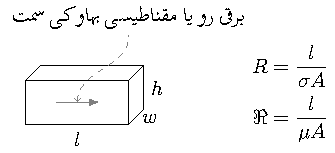
\includegraphics{figMagneticCircuitsResistanceAndReluctance}
\caption{مزاحمت اور ہچکچاہٹ}
\label{شکل_مقناطیسی_دور_مزاحمت_ہچکچاہٹ}
\end{figure}
اگر اس سلاخ کا \اصطلاح{مقناطیسی مستقل}\فرہنگ{مقناطیسی مستقل}\حاشیہب{permeability, magnetic constant}\فرہنگ{permeability}\فرہنگ{magnetic constant}  \عددیء{\mu} ہو تو اس سلاخ کی \اصطلاح{ہچکچاہٹ}\فرہنگ{ہچکچاہٹ}\فرہنگ{reluctance}\حاشیہب{reluctance} \عددیء{\Re}  یوں بیان کی جائے گی۔
\begin{align}\label{مساوات_مقناطیسی_دور_ہچکچاہٹ_کی_تعریف}
\Re = \frac{l}{\mu A}
\end{align}
مقناطیسی مستقل \عددیء{\mu} کو عموماً خالی خلاء کی مقناطیسی مستقل \عددیء{\mu_0} کی نسبت سے لکھا جاتا ہے یعنی
\begin{align}
\mu=\mu_r \mu_0
\end{align}
جہاں \عددیء{\mu_r} \اصطلاح{جزو مقناطیسی مستقل}\فرہنگ{مقناطیسی مستقل!جزو}\فرہنگ{relative permeability}\فرہنگ{permeability!relative}  کہلاتی ہے۔ہچکچاہٹ کی اکائی \اصطلاح{ایمپیئر-چکر فی ویبر}  ہے جس کی وضاحت جلد کی جائے گی۔
%
\ابتدا{مثال}
شکل  میں دی گئی سلاخ کی ہچکچاہٹ معلوم کریں
\عددیء{\mu_r=2000 }، \عددیء{l=\SI{10}{\centi \meter}}، \عددیء{h=\SI{3}{\centi \meter}} اور \عددیء{w=\SI{2.5}{\centi \meter}} ہیں۔

حل:
\begin{align*}
\Re& = \frac{l}{\mu_r \mu_0 A}\\
&=\frac{10\times 10^{-2}}{2000 \times 4 \pi \times 10^{-7} \times 2.5 \times 10^{-2} \times 3 \times 10^{-2}}\\
&=\SI{53044}{\ampere \cdot turns \per \weber}
\end{align*}
\انتہا{مثال}

\حصہ{کثافتِ برقی رو  اور برقی میدان کی شدت}\شناخت{حصہ_برقی_دور_کثافت_برقی_رو_اور_میدان}
اگر اس سلاخ کے سروں پر برقی دباؤ \عددیء{v} لاگو کی جائے جیسا کہ شکل  \حوالہ{شکل_مقناطیسی_دور_کثافت_رو_اور_برقی_شدت} میں دکھایا گیا ہے تو اس میں برقی رو \عددیء{i} گزرے گا جس کی مقدار \اصطلاح{اوہم} کے قانون\فرہنگ{قانون!اوہم}\حاشیہب{Ohm's law}\فرہنگ{Ohm's law}  سے یوں حاصل ہوتی ہے
\begin{align}
i=\frac{v}{R}
\end{align}
اس مساوات کو مساوات \حوالہ{مساوات_مقناطیسی_دور_مزاحمت_کی_تعریف}  کی مدد سے یوں لکھ سکتے ہیں
\begin{align}
i=v \left(\frac{\sigma A}{l}\right)
\end{align}
یا
\begin{align}
\frac{i}{A}=\sigma \left(\frac{v}{l} \right)
\end{align}
اسے مزید یوں لکھ سکتے ہیں
\begin{align}\label{مساوات_مقناطیسی_دور_اوہم_قانون_کی_تفرق_شکل}
J =\sigma E
\end{align}
جہاں 
\begin{align}
J&=\frac{i}{A} \label{مساوات_مقناطیسی_دور_کثافت_رو}\\
\intertext{اور}
E&=\frac{v}{l} \label{مساوات_مقناطیسی_دور_برقی_شدت}
\end{align}
کے برابر ہے۔

اگر شکل میں سمتیہ \سمتیہ{J} کا طول \عددیء{J} ہو اور سمتیہ \سمتیہ{E} کا طول \عددی{E} ہو جہاں ان دونوں سمتیہ کی سمت  \عددیء{\ay} ہے تب مساوات \حوالہ{مساوات_مقناطیسی_دور_اوہم_قانون_کی_تفرق_شکل} کو یوں لکھا جا سکتا ہے۔
\begin{align}
\kvec{J}=\sigma \kvec{E}
\end{align}
یہ مساوات اوہم کے قانون کی ایک اور شکل ہے۔ 

%
\begin{figure}
\centering
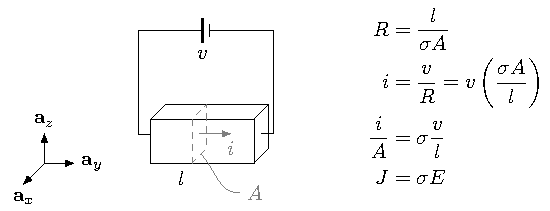
\includegraphics{figMagneticCircuitsCurrentDensityAndElectricFieldIntensity}
\caption{کثافتِ برقی رو اور برقی دباؤ کی شدت}
\label{شکل_مقناطیسی_دور_کثافت_رو_اور_برقی_شدت}
\end{figure}

شکل سے واضح ہے کہ برقی رو \عددیء{i} سلاخ کی رقبہ عمودی تراش \عددیء{A} سے گزرتی ہے لہٰذا مساوات \حوالہ{مساوات_مقناطیسی_دور_کثافت_رو} کے تحت \عددیء{J} برقی رو کی کثافت کو ظاہر کرتی ہے۔ اسی وجہ سے \عددیء{J} کو \اصطلاح{کثافتِ برقی رو}\فرہنگ{کثافت!برقی رو}\حاشیہب{current density} ہی کہتے ہیں۔ اسی طرح مساوات \حوالہ{مساوات_مقناطیسی_دور_برقی_شدت}   سے یہ واضح ہے کہ \عددیء{E} برقی دباؤ فی اکائی لمبائی کو ظاہر کرتی ہے۔  یوں  \عددیء{E} کو \اصطلاح{برقی میدان کی شدت}\فرہنگ{برقی میدان!شدت}\حاشیہب{electric field intensity} کہتے ہیں۔جہاں متن سے واضح ہو کہ برقی میدان کی بات ہو رہی ہے وہاں اس نام کو چھوٹا کر کے \عددیء{E} کو \اصطلاح{میدانی شدت}  سے پکارا جاتا ہے۔

	ہم بالکل اسی طرح مقناطیسی متغیرہ کے لئے بھی اس طرح کے مساوات لکھ سکتے ہیں۔ حصہ \حوالہ{حصہ_برقی_دور_کثافت_مقناطیسی_بہاو_اور_میدان}  میں ہم یہی کریں گے۔

\حصہ{برقی ادوار}
	برقی دور میں \اصطلاح{برقی دباؤ}\فرہنگ{برقی دباؤ}\حاشیہب{electric voltage}  \عددیء{v}\حاشیہد{برقی دباؤ کی اکائی وولٹ ہے جو اٹلی کے الِسانڈرو وولٹا کے نام ہے جنہوں نے برقی بیٹری ایجاد کی۔}  کی وجہ سے \اصطلاح{برقی رو}\فرہنگ{برقی رو}\حاشیہب{electric current} \عددیء{i} \حاشیہد{برقی رو کی اکائی ایمپیئر ہے جو فرانس کے انڈرِ میرِ ایمپیئر کے نام ہے جن کا برقی و مقناطیسی میدان میں اہم کردہر ہے۔} پیدا ہوتی ہے۔ تانبا\فرہنگ{تانبا}\حاشیہب{copper}   کی موصلیت \عددیء{\sigma=\SI{5.9e7}{\siemens \per \meter}} ہے جہاں \عددیء{\si{\siemens \per \meter}} موصلیت کی اکائی ہے۔لہٰذا تانبا کی بنی تار کی مزاحمت\حاشیہد{مزاحمت کی اکائی اوہم ہے جو جرمنی کے جارج سائمن اوہم کے نام ہے جنہوں نے قانونِ اوہم دریافت کیا۔}  \عددیء{R_{\textup{تار}}}  قابلِ نظرانداز ہوتی ہے۔اگر ایسی تار میں برقی رو \عددیء{i} کا گزر ہو  تو اس تار کی مزاحمت میں اوہم کے قانون کے تحت  برقی دباؤ  \عددیء{\Delta v=i R_{\textup{تار}}} گھٹے  گی۔\عددیء{R_{\textup{تار}}} کی قابلِ نظر انداز ہونے کی وجہ سے \عددیء{\Delta v} بھی قابلِ نظر انداز ہو گا یعنی \عددیء{\Delta v \to 0} لیا جا سکتا ہے۔ 

شکل \حوالہ{شکل_مقناطیسی_دور_سلسہ_وار_مزاحمتی_ادوار}-الف میں ایک ایسا ہی برقی دور دکھایا گیا ہے جس  میں تار کی مزاحمت کو اکٹھے کر کے ایک ہی جگہ  \عددیء{R_{\textup{تار}}} دکھایا گیا ہے۔ہم  اس دور کے لئے لکھ سکتے ہیں۔
\begin{align}
v&=\Delta v+v_L
\end{align}
تار میں برقی گھٹاو \عددیء{\Delta v} نظرانداز کرتے ہوئے
\begin{align}
v&=v_L
\end{align}
حاصل ہوتا ہے۔اس کا مطلب ہے کہ اگر تار میں برقی دباؤ کی گھٹاو قابل نظرانداز ہو تو لاگو برقی دباؤ جوں کے توں مزاحمت \عددیء{R_L} تک پہنچائی جا سکتی ہے۔برقی ادوار حل کرتے ہوئے یہی حقیقت بروئے کار لاتے ہوئے تار میں برقی دباؤ کے گھٹاو کو نظرانداز کیا جاتا ہے۔شکل \حوالہ{شکل_مقناطیسی_دور_سلسہ_وار_مزاحمتی_ادوار}-الف میں ایسا کرنے سے  شکل \حوالہ{شکل_مقناطیسی_دور_سلسہ_وار_مزاحمتی_ادوار}-ب حاصل ہوتا ہے۔یہاں یہ سمجھ لینا ضروری ہے کہ برقی تار کو اس غرض سے استعمال کیا جاتا ہے کہ لاگو برقی دباؤ کو جگہ استعمال تک بغیر گھٹائے پہنچایا جائے۔
\begin{figure}
\centering
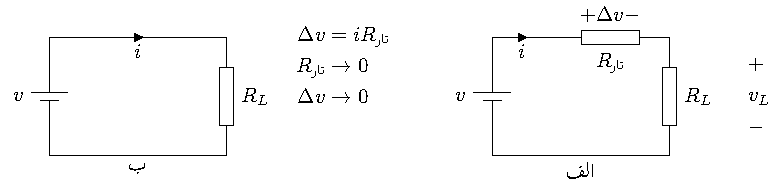
\includegraphics[width=\linewidth]{figMagneticCircuitsResistiveSeriesCircuit}
\caption{برقی دور میں تار کی مزاحمت کو نظر انداز کیا جاتا ہے۔}
\label{شکل_مقناطیسی_دور_سلسہ_وار_مزاحمتی_ادوار}
\end{figure}
%---------------------
\begin{figure}
\centering
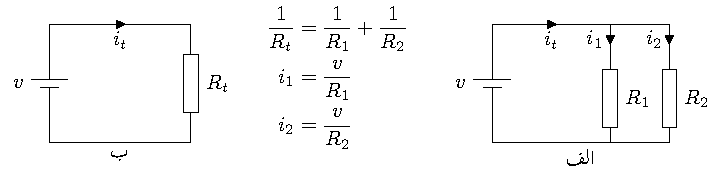
\includegraphics{figMagneticCircuitsResistiveParallelCircuit}
\caption{برقی رو کم مزاحمت کے راستے  زیادہ ہوتی ہے}
\label{شکل_مقناطیسی_دور_متوازی_مزاحمتی_دور}
\end{figure}
%

شکل \حوالہ{شکل_مقناطیسی_دور_متوازی_مزاحمتی_دور}  میں ایک اور مثال دی گئی ہے۔ یہاں ہم دیکھتے ہیں کہ برقی رو اس راستے زیادہ ہوتی ہے جس کی مزاحمت کم ہو۔ لہٰذا اگر \عددیء{R_1 < R_2}ہو تو \عددیء{i_1>i_2} ہو گی۔

\حصہ{مقناطیسی دور حصہ اول}
مقناطیسی دور بالکل برقی دور کی طرح ہوتے ہیں۔ بس ان میں برقی دباؤ \عددیء{v} کی جگہ \اصطلاح{مقناطیسی دباؤ}\فرہنگ{مقناطیسی دباؤ}\حاشیہب{magnetomotive force, mmf}\فرہنگ{mmf} \عددیء{\tau} ، برقی رو \عددیء{i}  کی جگہ \اصطلاح{مقناطیسی بہاو}\فرہنگ{مقناطیسی بہاو}\حاشیہب{flux}\فرہنگ{flux} \عددیء{\phi}  اور مزاحمت \عددیء{R} کی جگہ  \اصطلاح{ہچکچاہٹ}\فرہنگ{ہچکچاہٹ}\حاشیہب{reluctance}  \عددیء{\Re} ہوتی ہے۔ لہٰذا ہم بالکل ایک برقی دور کی طرح ایک مقناطیسی دور بنا سکتے ہیں۔ ایسا ہی ایک دور شکل \حوالہ{شکل_مقناطیسی__مقناطیسی_سلسلہ_وار_دور}-الف میں دکھایا گیا ہے۔
\begin{figure}
\centering
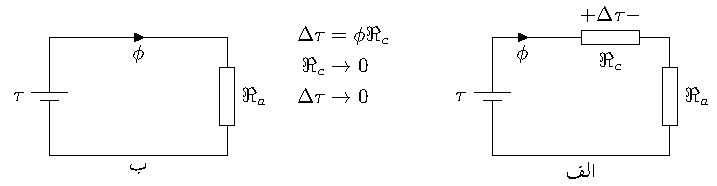
\includegraphics{figMagneticCircuitsReluctanceSeriesCircuit}
\caption{مقناطیسی دور}
\label{شکل_مقناطیسی__مقناطیسی_سلسلہ_وار_دور}
\end{figure}
%
یہاں بھی کوشش یہی ہے کہ کسی طرح مقناطیسی دباؤ \عددیء{\tau} کو بغیر کم کئے ہچکچاہٹ \عددیء{\Re_a} تک پہنچایا جائے۔ عموماً \عددیء{\Re_a} خلائی درز کی ہچکچاہٹ ہوتی ہے اور \عددیء{\Re_c} مقناطیسی مرکز کی۔ یہاں بھی اگر \عددیء{\Re_c} کو نظرانداز کرنا ممکن ہو تو ہمیں شکل \حوالہ{شکل_مقناطیسی__مقناطیسی_سلسلہ_وار_دور}-ب ملتا ہے جس میں مقناطیسی بہاو \عددیء{\phi} کو، بالکل اوہم کے قانون کی طرح
\begin{align}
\tau=\phi \Re_a
\end{align}
لکھ کر حاصل کیا جا سکتا ہے۔اگر \عددیء{\Re_c} کو نظرانداز کرنا ممکن نہ ہو تب بالکل سلسلہ وار مزاحمتوں کی طرح ہم اس شکل میں دیئے گئے دو سلسلہ وار ہچکچاہٹوں کا مجموعہ ہچکچاہٹ  \عددیء{\Re_s} کو استعمال کر کے برقی رو کا حساب لگائیں گے، یعنی
\begin{align}
\Re_s&=\Re_a+\Re_c\\
\tau&=\phi \Re_s \label{مساوات_مقناطیسی_دور_مقناطیسی_اوہم_قانون}
\end{align}
	بالکل برقی مثال کی طرح، مقناطیسی دباؤ کو کم ہچکچاہٹ والے راستے سے اس جگہ پہنچایا جاتا ہے جہاں اس کی ضرورت ہو۔ مساوات \حوالہ{مساوات_مقناطیسی_دور_ہچکچاہٹ_کی_تعریف}  سے ہم دیکھتے ہیں کہ ہچکچاہٹ،  مقناطیسی مستقل \عددیء{\mu} پر منحصر ہے ۔مقناطیسی مستقل کی اکائی\حاشیہب{Henry per meter}  ہینری فی میٹر \عددیء{\si{\henry \per \meter}} ہے۔\عددیء{\mu} کو عموماً \عددیء{\mu=\mu_r \mu_0} لکھا جاتا ہے جہاں  \عددیء{\mu_0=4 \pi \times 10^{-7}} ہینری فی میٹر کے برابر ہے اور \عددیء{\mu_r} کو \اصطلاح{جزو مقناطیسی مستقل}\فرہنگ{مقناطیسی مستقل!جزو}\حاشیہب{relative permeability, relative magnetic constant} کہتے ہیں۔ لوہا،  کچھ دھاتیں اور چند جدید مصنوعی اشیاء  ایسی ہیں جن کی \عددیء{\mu_r} کی قیمت \عددیء{\num{2000}} اور \عددیء{\num{80000}} کے  درمیان پائی جاتی ہیں۔ لہٰذا مقناطیسی دباؤ  ایک جگہ سے دوسری جگہ منتقل کرنے کے لئے انہی مقناطیسی اشیاء کو  استعمال کیا جاتا ہے۔ بد قسمتی سے ان مقناطیسی اشیاء کے  \عددیء{\mu} کی مقدار اتنی زیادہ  نہیں ہوتی کہ ان سے بنی سلاخ کی ہچکچاہٹ ہر جگہ نظرانداز کی جا سکے۔ مساوات \حوالہ{مساوات_مقناطیسی_دور_ہچکچاہٹ_کی_تعریف}  سے ہم دیکھتے ہیں کہ ہچکچاہٹ کم سے کم کرنے کی خاطر رقبہ عمودی تراش زیادہ سے زیادہ اور لمبائی کم سے کم  کرنی ہو گی۔ لہٰذا عموماً مقناطیسی دباؤ منتقل کرنے کے لئے ایک باریک تار نہیں بلکہ خاصی زیادہ رقبہ عمودی تراش کا مقناطیسی راستہ  درکار ہوتا ہے۔مقناطیسی مشین، مثلاً موٹر اور ٹرانسفارمر، کا بیشتر حصہ مقناطیسی دباؤ منتقل کرنے والے ان مقناطیسی اشیاء  پر ہی مشتمل ہوتا ہے۔ایسے مشینوں کے مرکز میں عموماً یہی مقناطیسی اشیاء پائے جاتے ہیں۔اسی وجہ سے  جن اشیاء کو اس مقصد کے لئے  استعمال کیا جاتا ہے انہیں \اصطلاح{مقناطیسی مرکز}\فرہنگ{مقناطیسی مرکز}\حاشیہب{magnetic core}\فرہنگ{magnetic core} کہتے ہیں۔برقی مشینوں میں استعمال  مقناطیسی مرکز لوہے کی باریک چادر یا پتری\فرہنگ{پتری}\حاشیہب{laminations}\فرہنگ{laminations}  تہہ  در تہہ رکھ کر بنائی جاتی ہے۔ مقناطیسی مرکز کے بارے میں حصہ \حوالہ{حصہ_مقناطیسی_دور_مقناطیسی_مادہ_کے_خصوصیات}  میں مزید معلومات فراہم کی جائے گی۔

\حصہ{کثافتِ مقناطیسی بہاو  اور مقناطیسی میدان کی شدت}\شناخت{حصہ_برقی_دور_کثافت_مقناطیسی_بہاو_اور_میدان}
حصہ \حوالہ{حصہ_برقی_دور_کثافت_برقی_رو_اور_میدان}  میں ہم نے برقی دور کی مثال دی تھی۔یہاں شکل \حوالہ{شکل_مقناطیسی__کثافت_مقناطیسی_بہاو_اور_شدت} میں ایک مقناطیسی دور کی  مثال دیتے ہیں۔یہاں مقناطیسی مرکز کی \عددیء{\mu_r = \infty} تصور کی گئی ہے لہٰذا اس مرکز کی ہچکچاہٹ \عددیء{\Re_c} صفر ہو گی۔ لہٰذا جیسے حصہ \حوالہ{حصہ_برقی_دور_کثافت_برقی_رو_اور_میدان}   میں تانبا کی تار استعمال کی گئی تھی یہاں اسی طرح مقناطیسی مرکز کو مقناطیسی دباؤ \عددیء{\tau} ایک جگہ سے دوسری جگہ منتقل کرنے کے لئے استعمال کیا گیا ہے۔ اس شکل میں مقناطیسی دباؤ کو خلائی درز کی ہچکچاہٹ \عددیء{\Re_a} تک پہنچایا گیا ہے۔
\begin{figure}
\centering
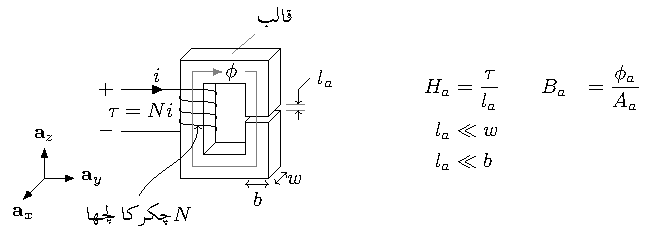
\includegraphics{figMagneticCircuitsMagneticFluxDensityAndIntensity}
\caption{کثافتِ مقناطیسی بہاو اور مقناطیسی میدان کی شدت۔}
\label{شکل_مقناطیسی__کثافت_مقناطیسی_بہاو_اور_شدت}
\end{figure}
لہٰذا یہاں کُل ہچکچاہٹ صرف خلائی درز کی ہچکچاہٹ ہی ہے یعنی
\begin{align}
\Re_a=\frac{l_a}{\mu_0 A_z}
\end{align}
اگر خلائی درز کی لمبائی \عددیء{l_a} مرکز کے رقبہ عمودی تراش کے اطراف \عددیء{b} اور \عددیء{w} سے نہایت کم ہو یعنی \عددیء{l_a \ll b} اور \عددیء{l_a \ll w} تب خلائی درز کے رقبہ عمودی تراش \عددیء{A_a} کو مرکز کے رقبہ عمودی تراش \عددیء{\Re_c} کے برابر لیا جاتا ہے یعنی
\begin{align}
A_a=A_c=w b
\end{align}
 اس کتاب میں جہاں بتلایا نہ گیا ہو وہاں \عددیء{l_a \ll b} اور \عددیء{l_a \ll w} تصور کرتے ہوئے \عددیء{A_a=A_c} لیا جائے گا۔
 
مقناطیسی دباؤ کو یوں بیان کیا جاتا ہے
\begin{align}
\tau=N i
\end{align}
یعنی برقی تار کے چکر ضربِ ان میں برقی رو۔ لہٰذا مقناطیسی دباؤ کی اکائی \اصطلاح{ایمپیئر-چکر}\فرہنگ{ایمپیئر-چکر}\حاشیہب{ampere-turn}\فرہنگ{ampere-turn}  ہے۔ بالکل حصہ \حوالہ{حصہ_برقی_دور_کثافت_برقی_رو_اور_میدان}   کی طرح ہم مساوات \حوالہ{مساوات_مقناطیسی_دور_مقناطیسی_اوہم_قانون} کو یوں لکھ سکتے ہیں۔
\begin{align}\label{مساوات_مقناطیسی_ڈور_بہاو_مساوی_دباؤ_بٹا_ہچکچاہٹ}
\phi_a=\frac{\tau}{\Re_a}
\end{align}
مقناطیسی بہاو کی اکائی \اصطلاح{ویبر}\فرہنگ{ویبر}\حاشیہب{Weber}\فرہنگ{Weber}\حاشیہد{یہ اکائی جرمنی کے ولیم اڈورڈ ویبر کے نام ہے جن کا برقی و مقناطیسی میدان میں اہم کردہر رہا ہے}  ہے اور ہچکچاہٹ کی اکائی \اصطلاح{ایمپیئر-چکر فی ویبر}\حاشیہب{ampere-turn per weber} ہے۔  خلائی درز میں مقناطیسی بہاو \عددیء{\phi_a} اور مرکز میں مقناطیسی بہاو \عددیء{\phi_c} برابر ہیں۔ اس مساوات کو مساوات \حوالہ{مساوات_مقناطیسی_دور_ہچکچاہٹ_کی_تعریف}   کی مدد سے یوں لکھ سکتے ہیں۔
\begin{align}
\phi_a &=\tau \left(\frac{\mu_0 A_a}{l_a} \right) \nonumber \\
\intertext{یا}
\frac{\phi_a}{A_a}&=\mu_0 \left( \frac{\tau}{l_a} \right) \label{مساوات_مقناطیسی_دور_کثافت_بہاو_اوہم_قانون_سے}
\end{align}
	اس مساوات میں بائیں جانب مقناطیسی بہاو فی اکائی رقبہ کو \اصطلاح{کثافتِ مقناطیسی بہاو}\فرہنگ{مقناطیسی بہاو!کثافت}\حاشیہب{magnetic flux density}\فرہنگ{magnetic flux!density} \عددیء{B_a} اور دائیں جانب مقناطیسی دباؤ فی اکائی لمبائی کو \اصطلاح{مقناطیسی میدان کی شدت}\فرہنگ{مقناطیسی میدان!شدت}\حاشیہب{magnetic field intensity}\فرہنگ{magnetic field!intensity}  \عددیء{H_a} لکھا جا سکتا ہے۔یعنی
\begin{align}
B_a&=\frac{\phi_a}{A_a}\\
H_a&=\frac{\tau}{l_a}
\end{align}
کثافتِ مقناطیسی بہاو کی اکائی \اصطلاح{ویبر فی مربع میٹر} ہے جس کو \اصطلاح{ٹسلا}\فرہنگ{ٹسلا}\فرہنگ{Tesla}\حاشیہد{Tesla:  یہ اکائی سربیا کے نِکولا ٹسلا کے نام ہے جنہوں نے بدلتی رو برقی طاقت عام کرنے میں اہم کردہر ادا کیا}  کا نام دیا گیا ہے۔مقناطیسی میدان کی شدت کی اکائی \اصطلاح{ایمپیئر فی میٹر}\حاشیہب{ampere per meter}  ہے۔ لہٰذا مساوات \حوالہ{مساوات_مقناطیسی_دور_کثافت_بہاو_اوہم_قانون_سے} کو ہم یوں لکھ سکتے ہیں۔
\begin{align}
B_a=\mu_0 H_a
\end{align}
جہاں متن سے واضح ہو کہ مقناطیسی میدان کی بات ہو رہی ہے وہاں مقناطیسی میدان کی شدت کو \اصطلاح{میدانی شدت}\حاشیہب{field intensity} کہا جاتا ہے۔  شکل میں ہم دیکھتے ہیں کہ خلائی درز میں مقناطیسی بہاو کی سمت،  اکائی سمتیہ \عددیء{\az} کی الٹ سمت میں ہے لہٰذا ہم کثافتِ مقناطیسی بہاو کو \عددیء{\kvec{B_a}=-B_a \az} لکھ سکتے ہیں۔ اسی طرح خلائی درز میں مقناطیسی دباؤ  اکائی سمتیہ \عددیء{\az} کی الٹ سمت میں دباؤ ڈال رہی ہے لہٰذا ہم مقناطیسی دباؤ کی شدت کو \عددیء{\kvec{H_a}=-H_a \az} لکھ سکتے ہیں۔ لہٰذا اس مساوات کو یوں لکھا جا سکتا ہے۔
\begin{align}
\kvec{B_a}=\mu_0 \kvec{H_a}
\end{align}
اگر خلاء کی جگہ کوئی اور مادہ ہو، تب ہم اس مساوات کو یوں لکھتے
\begin{align}
\kvec{B}=\mu \kvec{H}
\end{align}
%
\ابتدا{مثال}
شکل \حوالہ{شکل_مقناطیسی__کثافت_مقناطیسی_بہاو_اور_شدت} میں خلائی درز میں کثافتِ مقناطیسی بہاو \عددیء{0.1} ٹسلا درکار ہے۔مرکز کی \عددیء{\mu_r=\infty}  ہے اور خلائی درز کی لمبائی \عددیء{1} ملی میٹر ہے۔اگر  مرکز کے گرد برقی تار کے \عددیء{100} چکر ہوں تو ان میں درکار برقی رو معلوم کریں۔

حل:
\begin{align*}
\tau&=\phi \Re\\
N i & \phi \left(\frac{l}{\mu_0 A} \right)\\
\frac{\phi}{A}&=\frac{ N i \mu_0}{l}
\end{align*}
لہٰذا
\begin{align*}
0.1&=\frac{100 \times i \times 4 \pi  10^{-7}}{0.001}\\
i&=\frac{0.1 \times 0.001}{100 \times 4 \pi  10^{-7}}=\SI{0.79567}{\ampere}
\end{align*}
یعنی \عددیء{0.79567} ایمپیئر برقی رو سے خلائی درز میں \عددیء{0.1} ٹسلا کثافتِ مقناطیسی بہاو حاصل ہو جائے گی۔
\انتہا{مثال}
%
\حصہ{مقناطیسی دور حصہ دوم}
شکل \حوالہ{شکل_مقناطیسی__سادہ_مقناطیسی_دور_بغیر_درز} میں ایک سادہ مقناطیسی نظام دکھایا گیا ہے جس میں مرکز کی مقناطیسی مستقل کو محدود تصور کیا گیا ہے۔شکل میں مقناطیسی دباؤ  \عددیء{\tau=N i} مقناطیسی مرکز میں مقناطیسی بہاو \عددیء{\phi_c} کو جنم دیتی ہے۔ یہاں مرکز کا رقبہ عمودی تراش \عددیء{A_c}  ہر جگہ یکساں ہے اور مرکز  کی اوسط لمبائی \عددیء{l_c} ہے۔ مرکز میں مقناطیسی بہاو  کی سمت \اصطلاح{فلیمنگ}\حاشیہب{Fleming's right hand rule} کے دائیں ہاتھ کے قانون  سے معلوم کی جا سکتی ہے۔اس قانون کو دو طریقوں سے بیان کیا جا سکتا ہے۔
\begin{itemize}
\item
اگر ایک لچھے کو دائیں ہاتھ سے یوں پکڑا  جائے کہ ہاتھ کی چار انگلیاں لچھے میں برقی رو کی سمت میں لپٹی  ہوں تو انگوٹھا اُس مقناطیسی بہاو کی سمت میں ہو گا جو اس برقی رو کی وجہ سے وجود میں آئے گا۔
\item
اگر ایک تار جس میں برقی رو کا گزر ہو، کو دائیں ہاتھ سے یوں پکڑا جائے کہ انگوٹھا  برقی رو  کی سمت میں ہو تو باقی چار انگلیاں اُس مقناطیسی  بہاو کی سمت میں لپٹی ہوں گی  جو اس برقی رو کی وجہ سے  پیدا ہوگا۔
\end{itemize}

ان دو بیانات میں پہلا بیان،  لچھے میں مقناطیسی بہاو کی سمت معلوم کرنے کے لئے زیادہ آسان ثابت ہوتا ہے جبکہ کسی ایک سیدھی تار کے گرد مقناطیسی بہاو کی سمت دوسرے بیان سے زیادہ آسانی سے معلوم کی جا سکتی ہے۔
\begin{figure}
\centering
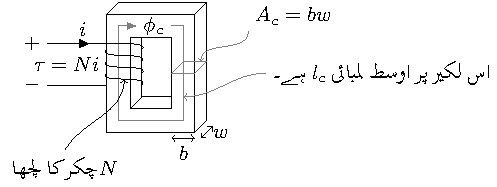
\includegraphics{figMagneticCircuitsSimpleMagneticCircuitNoGap}
\caption{سادہ مقناطیسی دور}
\label{شکل_مقناطیسی__سادہ_مقناطیسی_دور_بغیر_درز}
\end{figure}
لہٰذا مرکز میں مقناطیسی بہاو  گھڑی کے سمت میں ہے۔ مقناطیسی بہاو کو  شکل \حوالہ{شکل_مقناطیسی__سادہ_مقناطیسی_دور_بغیر_درز} میں تیر والے ہلکی سیاہی کے لکیر  سے ظاہر کیا گیا ہے۔ یہاں مرکز کی ہچکچاہٹ 
\begin{align*}
\Re_c&=\frac{l_c}{\mu_c A_c}
\end{align*}
لکھتے ہوئے مقناطیسی بہاو یوں
\begin{align*}
\phi_c&=\frac{\tau}{\Re_c}=N i \left(\frac{\mu_c A_c}{l_c} \right)
\end{align*}
حاصل کی جا سکتی ہے۔اس طرح ہم سب متغیرات حاصل کر سکتے ہیں۔
%
\ابتدا{مثال}
شکل \حوالہ{شکل_مقناطیسی__درز_اور_ہچکچاہٹ}  میں ایک مقناطیسی مرکز دکھایا گیا ہے جہاں
\begin{align}
\text{مرکز}= \left\{ 
  \begin{array}{l l}
  h=\SI{20}{\centi\meter} & m=\SI{10}{\centi \meter}\\
 n=\SI{8}{\centi\meter} & w=\SI{2}{\centi \meter}\\
 l_a=\SI{1}{\milli\meter} & \mu_r =40000 \\
 \end{array} \right.
\end{align}
ہیں۔مرکز اور خلائی درز کی ہچکچاہٹیں حاصل کریں۔
\begin{figure}
\centering
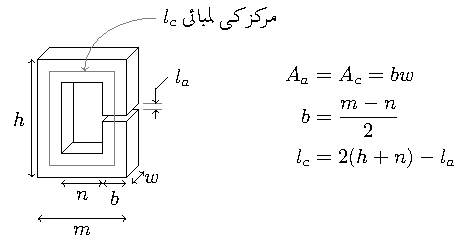
\includegraphics{figMagneticCircuitsCoreWithGapAndReluctance}
\caption{خلائی درز اور مرکز کے ہچکچاہٹ}
\label{شکل_مقناطیسی__درز_اور_ہچکچاہٹ}
\end{figure}
حل:
\begin{align*}
b&=\frac{m-n}{2}=\frac{0.1-0.08}{2}=\SI{0.01}{\meter}\\
A_a&=A_c=bw=0.01 \times 0.02=\SI{0.0002}{\square \meter}\\
l_c&=2(h+n)-l_a=2(0.2+0.08)-0.001=\SI{0.559}{\meter}
\end{align*}
%
\begin{align*}
\Re_c&=\frac{l_c}{\mu_r \mu_0 A_c}=\frac{0.559}{40000 \times 4 \pi 10^{-7} \times 0.0002}=\SI{55598}{\ampere \cdot t \per \weber}\\
\Re_a&=\frac{l_a}{\mu_0 A_a}=\frac{0.001}{4 \pi 10^{-7} \times 0.0002}=\SI{3978358}{\ampere \cdot t \per \weber}
\end{align*}
ہم دیکھتے ہیں اگرچہ مرکز کی لمبائی خلائی درز کی لمبائی سے \عددیء{559} گنا زیادہ ہے تب بھی خلائی درز کی ہچکچاہٹ \عددیء{71} گنا زیادہ ہے یعنی \عددیء{\Re_a  \gg \Re_c} 
\انتہا{مثال}
%
\ابتدا{مثال}
شکل  \حوالہ{شکل_مقناطیسی_دور_سادہ_گھومتا_مشین} سے رجوع کریں۔اگر ایک خلائی درز \عددیء{5} ملی میٹر لمبا ہو اور گھومتے حصہ پر \عددیء{1000} چکر ہوں تو خلائی درز میں \عددیء{0.95} ٹسلا کثافتِ برقی بہاو حاصل کرنے کی خاطر درکار برقی رو معلوم کریں۔
\begin{figure}
\centering
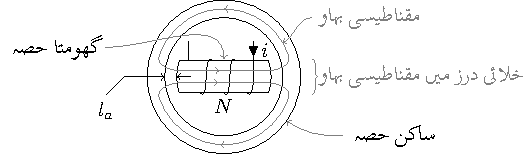
\includegraphics{figMagneticCircuitsSimpleRotatingMachineOutline}
\caption{سادہ گھومنے والا مشین}
\label{شکل_مقناطیسی_دور_سادہ_گھومتا_مشین}
\end{figure}
حل:
	 اس شکل میں ایک گھومتے مشین، مثلاً موٹر، کی ایک سادہ شکل دکھائی گئی ہے۔ ایسے آلوں میں باہر کا حصہ ساکن رہتا ہے جس کو مشین کا ساکن حصہ کہتے ہیں اور اس ساکن حصہ کے اندر اس کا ایک حصہ گھومتا ہے جسے گھومتا حصہ کہتے ہیں۔ اس مثال میں ان دونوں حصوں کا  \عددیء{\mu_r=\infty}  ہے لہٰذا ان کی ہچکچاہٹ صفر ہے۔ مقناطیسی بہاو  ہلکی سیاہی کے لکیر سے ظاہر کی گئی ہے۔ یہ خلائی درز میں سے، ایک مکمل چکر کے دوران، دو مرتبہ گزرتی ہے۔ یہ دو خلائی درز ہر لحاظ سے ایک جیسے ہیں لہٰذا ان دونوں خلائی درز کی ہچکچاہٹ بھی برابر ہوں گی۔مزید یہ کہ ان خلائی درز کی ہچکچاہٹ سلسلہ وار ہیں۔شکل میں مقناطیسی بہاو کو گھومتے حصہ سے ساکن حصہ کی طرف، خلائی درز سے گزرتے دکھایا گیا ہے۔خلائی درز کی لمبائی \عددیء{l_a} بہت کم ہے لہٰذا خلائی درز کا عمودی رقبہ تراش \عددیء{A_a} وہی ہو گا جو گھومتے حصہ کا ہے یعنی \عددیء{A_c} 

  ایک خلائی درز کی ہچکچاہٹ
\begin{align*}
\Re_a=\frac{l_a}{\mu_0 A_a}=\frac{l_a}{\mu_0 \A_c}
\end{align*}
ہے۔لہٰذا کُل ہچکچاہٹ ہو گی
\begin{align*}
\Re_s=\Re_a=\Re_a=\frac{2 l_a}{\mu_0 A_c}
\end{align*}
یوں خلائی درز میں مقناطیسی بہاو \عددیء{\phi_a} اور کثافتِ مقناطیسی بہاو \عددیء{B_a} یہ ہوں گے۔
\begin{align*}
\phi_a&=\frac{\tau}{\Re_s}=\left(N i \right) \left (\frac{\mu_0 A_c}{2 l_a} \right)\\
B_a&=\frac{\phi_a}{A_a}=\frac{\mu_0 N i}{2 l_a}
\end{align*}
اس مساوات میں اعداد استعمال کرتے ہیں
\begin{align*}
0.95&=\frac{4 \pi 10^{-7} \times 1000 \times i}{2 \times 0.005}\\
i&=\frac{0.95 \times 2 \times 0.005}{ 4 \pi 10^{-7} \times 1000}=\SI{7.56}{\ampere}
\end{align*}
موٹر اور جنریٹروں کی خلاء میں تقریباً ایک ٹسلا کثافتِ برقی بہاو ہوتی ہے۔
\انتہا{مثال}

\حصہ{خود امالہ  ، مشترکہ امالہ  اور توانائی}
مقناطیسی بہاو کی، وقت کے ساتھ تبدیلی، برقی دباؤ  کو جنم دیتی ہے۔ لہٰذا  اگر شکل \حوالہ{شکل_مقناطیسی__کثافت_مقناطیسی_بہاو_اور_شدت}  کے مرکز میں مقناطیسی بہاو تبدیل ہو رہی ہو تو اس کی وجہ سے اس کے لچھے میں برقی دباؤ پیدا ہو گا جو کہ اس لچھے کے سروں پر نمودار ہو گا۔ اِس طرح پیدا ہونے والی برقی دباؤ کو \اصطلاح{امالی برقی دباؤ}\فرہنگ{امالی برقی دباؤ}\حاشیہب{induced voltage}\فرہنگ{induced voltage}  کہتے ہیں۔ \اصطلاح{قانونِ فیراڈے}\فرہنگ{فیراڈے!قانون}\حاشیہب{Faraday's law}\فرہنگ{Faraday's law}  کے تحت\حاشیہد{مائکل فیراڈے انگلستانی سائنسدان تھے جنہوں نے محرک برقی دباؤ دریافت کی}
\begin{align}\label{مساوات_مقناطیسی_دور_فیراڈے_قانون}
e=N \frac{\partial \phi}{\partial t} =\frac{\partial \lambda}{\partial t}
\end{align}
اس مساوات میں ہم لچھے میں، وقت کے ساتھ تبدیل ہونے والی، مقناطیسی بہاو کو \عددیء{\phi} سے ظاہر کر رہے ہیں۔\عددیء{N \phi} کو لچھے کی \اصطلاح{ارتباط بہاو}\فرہنگ{ارتباط بہاو}\حاشیہب{flux linkage} \عددیء{\lambda}  کہتے ہیں جس کی اکائی \اصطلاح{ویبر-چکر}\فرہنگ{ویبر-چکر}\حاشیہب{weber-turn}  ہے۔ اس امالی برقی دباؤ  کی سمت کا تعین یوں کیا جاتا ہے کہ اگر دیئے گئے لچھے کی سروں کو \اصطلاح{کسرِ دور}\فرہنگ{کسر دور}\حاشیہب{short circuit}   کیا جائے تو اِس میں برقی رو اُس سمت میں ہو گی جس میں مقناطیسی بہاو کی تبدیلی کو روکا جا سکے۔ 

جن مقناطیسی دوروں میں مقناطیسی مستقل \عددیء{\mu}  کو اٹل مقدار تصور کیا جا سکے یا جن میں خلائی درز کی ہچکچاہٹ مرکز کی ہچکچاہٹ سے بہت زیادہ ہو یعنی \عددیء{\Re_a \gg \Re_c} ، ان حالات میں ہم لچھے کی  \اصطلاح{امالہ}\فرہنگ{امالہ}\حاشیہب{inductance}\فرہنگ{inductance} \عددیء{L}  کو یوں بیان کرتے ہیں۔
\begin{align}\label{مساوات_مقناطیسی_دور_خود_امالہ_تعریف}
L=\frac{\lambda}{i}
\end{align}

امالہ کی اکائی ویبر-چکر فی ایمپیئر ہے جس کو \اصطلاح{ہینری}\فرہنگ{Henry}\حاشیہب{Henry}\فرہنگ{Henry} \عددیء{H} کا نام\حاشیہد{امریکی سائنسدان جوزف ہینری جنہوں نے مائکل فیراڈے سے علیحدہ  طور پر محرک برقی دباؤ دریافت کی} دیا گیا ہے۔ لہٰذا
\begin{align}
L=\frac{N \phi}{i}=\frac{N B_c A_c}{i}=\frac{N^2 \mu_0 A_a}{l_a}
\end{align}
%
\ابتدا{مثال}
شکل \حوالہ{شکل_مقناطیسی__کثافت_مقناطیسی_بہاو_اور_شدت} میں اگر \عددیء{b=\SI{5}{\centi \meter},w=\SI{4}{\centi\meter},l_a=\SI{3}{\milli \meter}} جبکہ لچھے کے \عددیء{1000} چکر اور مرکز کی اوسط لمبائی \عددیء{l_c=\SI{30}{\centi\meter}} ہو تب ان دو صورتوں میں لچھے کی امالہ معلوم کریں۔
\begin{itemize}
\item
مرکز کی \عددیء{\mu_r = \infty} ہے۔
\item
مرکز کی \عددیء{\mu_r = 500} ہے۔
\end{itemize}

حل:
	پہلی صورت میں مرکز کی \عددیء{\mu_r=\infty} ہونے کی وجہ سے مرکز کی ہچکچاہٹ نظرانداز کی جا سکتی ہے۔یوں
\begin{align*}
L&=\frac{N^2 \mu_0 w b}{l_a}\\
&=\frac{1000^2 \times 4 \pi 10^{-7} \times 0.04 \times 0.05}{0.003}\\
&=\SI{0.838}{\henry}
\end{align*}
	دوسری صورت میں \عددیء{\mu_r=500} ہے۔یوں مرکز کی ہچکچاہٹ صفر نہیں۔خلاء اور مرکز کی ہچکچاہٹ پہلے دریافت کرتے ہیں
\begin{align*}
\Re_a&=\frac{l_a}{\mu_0 w b}=\frac{0.003}{4\pi 10^{-7} \times 0.04 \times 0.05}=\SI{1193507}{\ampere \cdot t \per \weber}\\
\Re_c&=\frac{l_c}{\mu_r \mu_0 w b}=\frac{0.3}{500 \times 4\pi 10^{-7} \times 0.04 \times 0.05}=\SI{238701}{\ampere \cdot t \per \weber}
\end{align*}
لہٰذا
\begin{align*}
\phi&=\frac{N i}{\Re_a+\Re_c}\\
\lambda &= N \phi = \frac{N^2 i}{\Re_a+\Re_c}\\
L&=\frac{\lambda}{i}=\frac{N^2}{\Re_a+\Re_c}=\frac{1000^2}{\num{1193507}+\num{238701}}=\SI{0.698}{\henry}
\end{align*}
\انتہا{مثال}
%
\ابتدا{مثال}
شکل \حوالہ{شکل_مقناطیسی_ادوار_پیچدار_لچھا} میں ایک پیچدار لچھا\فرہنگ{لچھا!پیچدار}\حاشیہب{spiral coil} دکھایا گیا ہے جس کی تفصیل یوں ہے

\عددیء{N=11, r=\SI{0.49}{\meter},l=\SI{0.94}{\meter}}

ایسے پیچدار لچھے کی بیشتر مقناطیسی بہاو لچھے کے اندر محوری سمت میں ہوتی ہے۔لچھے کے باہر مقناطیسی بہاو کی مقدار قابلِ نظرانداز ہوتی ہے۔یوں لچھے کے اندر محوری جانب مقناطیسی شدت
\begin{align*}
H=\frac{N i}{l}
\end{align*}
ہوتی ہے۔اس لچھے کی خود امالہ حاصل کریں۔
\begin{figure}
\centering
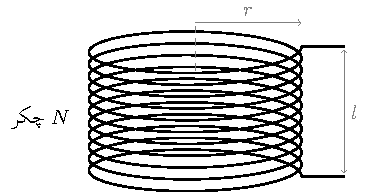
\includegraphics{figMagneticCircuitsCoil}
\caption{پیچدار لچھا}
\label{شکل_مقناطیسی_ادوار_پیچدار_لچھا}
\end{figure}
حل:
\begin{align*}
B&=\mu_0 H=\frac{\mu_0 N i}{l}\\
\phi&=B  \pi r^2=\frac{\mu_0 N i \pi r^2}{l}\\ 
\lambda&=N \phi =\frac{\mu_0 N^2 i \pi r^2}{l}\\ 
L&=\frac{\lambda}{i}=\frac{\mu_0 N^2 \pi r^2}{l}
\end{align*} 
یوں
\begin{align*}
L=\frac{4 \pi 10^{-7} \times 11^2 \times \pi  \times 0.49^2}{0.94}=\SI{122}{\micro \henry}
\end{align*}
یہ پیچدار لچھا میں نے  \عددیء{3000} کلو گرام لوہا پگھلانے والی بھٹی میں استعمال کیا ہے۔
\انتہا{مثال}
%
شکل \حوالہ{شکل_مقناطیسی_ادوار_دو_لچھے_ایک_درز} میں دو لچھے والا ایک مقناطیسی دور دکھایا گیا ہے۔ ایک لچھے کے  \عددیء{N_1} چکر ہیں اور اس میں برقی رو \عددیء{i_1} ہے اور دوسرا لچھا \عددیء{N_2} چکر کا ہے اور اس میں برقی  رو \عددیء{i_2} ہے۔ دونوں لچھوں میں برقی رو کی سمتیں یوں ہیں کہ اِن  دونوں کا مقناطیسی دباؤ جمع ہو۔ یوں اگر مرکز کے امالہ کو نظرانداز کیا جائے تو ہم مقناطیسی بہاو \عددیء{\phi} کے لئے لکھ سکتے ہیں
\begin{align}
\phi=\left (N_1 i_1 +N_2 i_2 \right ) \frac{\mu_0 A_a}{l_a}
\end{align} 
%
\begin{figure}
\centering
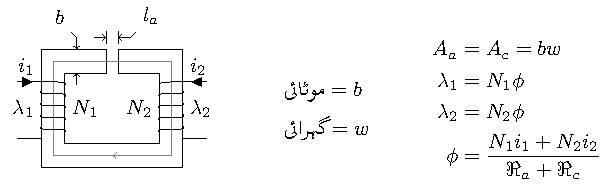
\includegraphics{figMagneticCircuitsTwoCoilsWithGap}
\caption{دو لچھے والا مقناطیسی دور۔}
\label{شکل_مقناطیسی_ادوار_دو_لچھے_ایک_درز}
\end{figure}
یہاں \عددیء{\phi} دونوں لچھوں کے مجموعی مقناطیسی دباؤ یعنی \عددیء{N_1 i_1+N_2 i_2} سے پیدا ہونے والا مقناطیسی بہاو ہے۔ اس مقناطیسی بہاو  کی ان  لچھوں  کے ساتھ  ارتباط کو یوں لکھا جا سکتا ہے۔
\begin{align}
\lambda_1=N_1 \phi=N_1^2  \frac{\mu_0 A_a}{l_a} i_1 +N_1 N_2  \frac{\mu_0 A_a}{l_a} i_2
\end{align}
اس کو یوں لکھا جا سکتا ہے
\begin{align}\label{مساوات_مقناطیسی_دور_ارتباط_دو_لچھے}
\lambda_1 = L_{11} i_1+L_{12} i_2
\end{align}
جہاں
\begin{align}
L_{11}&=N_1^2  \frac{\mu_0 A_a}{l_a}\\
L_{12}&=N_1 N_2  \frac{\mu_0 A_a}{l_a}
\end{align}
ہیں۔ یہاں \عددیء{L_{11}} پہلے لچھے کی  \اصطلاح{خود امالہ}\فرہنگ{خود امالہ}\حاشیہب{self inductance}\فرہنگ{self inductance}  ہے اور  \عددیء{L_{11} i_1} اِس لچھے کی اپنے برقی رو \عددیء{i_1} سے پیدا مقناطیسی بہاو  کے ساتھ  ارتباط بہاو ہے جسے \اصطلاح{خود ارتباط بہاو}\فرہنگ{خود ارتباط بہاو}\حاشیہب{self flux linkage}\فرہنگ{self flux linkage} کہتے ہیں۔\عددیء{L_{12}}  اِن دونوں لچھوں  کا  \اصطلاح{مشترکہ امالہ}\فرہنگ{مشترکہ امالہ}\حاشیہب{mutual inductance}\فرہنگ{mutual inductance} ہے اور  \عددیء{L_{12} i_2}  لچھا نمبر-1  کے ساتھ برقی رو  \عددیء{i_2} کی وجہ سے  ارتباط بہاو  ہے جسے \اصطلاح{مشترکہ ارتباط بہاو}\فرہنگ{مشترکہ ارتباط امالہ}\حاشیہب{mutual flux linkage}\فرہنگ{mutual flux linkage}  کہتے ہیں ۔ بالکل اسی طرح ہم دوسرے لچھے کے لئے لکھ سکتے ہیں
\begin{align}
\lambda_2&=N_2 \phi=N_2 N_1 \frac{\mu_0 A_a}{l_a} i_1+N_2^2 \frac{\mu_0 A_a}{l_a} i_2  \nonumber \\
&=L_{21} i_1+L_{22} i_2 \label{مساوات_مقناطیسی_دور_دوسرے_لچھے_کی_ارتباط}
\end{align}
جہاں
\begin{align}
L_{22}&=N_2^2 \frac{\mu_0 A_a}{l_a}\\
L_{21}&=L_{12}=N_2 N_1 \frac{\mu_0 A_a}{l_a} \label{مساوات_مقناطیسی_دور_مشترکہ_امالہ_یکساں}
\end{align}
ہیں۔\عددیء{L_{22}} دو نمبر لچھے  کی خود امالہ اور  \عددیء{L_{21}=L_{12}} ان  دو لچھوں کی مشترکہ امالہ ہے۔ یہاں یہ واضح کرنا ضروری ہے کہ امالہ کا تصور اس وقت کارآمد ہوتا جب ہم مقناطیسی مستقل \عددیء{\mu}  کو اٹل تصور کر سکیں۔

مساوات \حوالہ{مساوات_مقناطیسی_دور_خود_امالہ_تعریف}  کو مساوات \حوالہ{مساوات_مقناطیسی_دور_فیراڈے_قانون}  میں استعمال کریں تو 
\begin{align}
e=\frac{\partial \lambda}{\partial t}=\frac{ \partial \left (N \phi \right)}{\partial t}=\frac{\partial \left( L i\right) }{\partial t}
\end{align}
اگر امالہ مقررہ ہو جیسا کہ ساکن آلوں میں ہوتا ہے تب ہمیں  امالہ کی جانی پہچانی مساوات ملتی ہے 
\begin{align}
e=L \frac{\partial i}{\partial t}
\end{align}
مگر اگر امالہ بھی تبدیل ہو جیسا کہ موٹروں اور جنریٹروں میں ہوتا ہے تب
\begin{align}
e= L \frac{\partial i}{\partial t} + i \frac{\partial L}{\partial t}
\end{align}
توانائی\فرہنگ{توانائی}\حاشیہب{energy}\فرہنگ{energy}  کی اکائی \اصطلاح{جاول}\فرہنگ{جاول}\حاشیہب{Joule}\فرہنگ{Joule} \عددیء{J}\حاشیہد{جیمس پریسقوٹ جاول انگلستانی سائنسدان جنہوں نے حرارت اور میکانی کام کا رشتہ دریافت کیا} ہے اور طاقت\فرہنگ{طاقت}\حاشیہب{power}\فرہنگ{power}  کی اکائی\حاشیہد{سکاٹلینڈ کے جیمز واٹ جنہوں نے بخارات پر چلنے والے انجن پر کام کیا} جاول فی سیکنڈ یا \اصطلاح{واٹ}\فرہنگ{واٹ}\حاشیہب{Watt}\فرہنگ{Watt} \عددیء{W}  ہے۔

اس کتاب میں توانائی یا کام کو \عددیء{W} سے ظاہر کیا جائے گا مگر طاقت کی اکائی واٹ \عددیء{W} کے لئے بھی ہی کی علامت استعمال ہوتی ہے۔امید کی جاتی ہے کہ اس سے غلطی پیش نہیں آئے گی اور استعمال کو دیکھ کر یہ فیصلہ کرنا کہ اس کا کونسا مطلب لیا جا رہا ہے دشوار نہ ہو گا۔

وقت کے ساتھ توانائی کی شرح کو طاقت کہتے ہیں لہٰذا کسی لچھے کے لئے ہم لکھ سکتے ہیں
\begin{align}
p=\frac{\dif W}{\dif t} = e i = i \frac{\partial \lambda}{\partial t}
\end{align} 
لہٰذا ایک مقناطیسی دور میں  \عددیء{t_1} سے \عددیء{t_2} تک کے وقفے میں مقناطیسی توانائی میں تبدیلی کو تکمل کے ذریعہ یوں حاصل کیا جا سکتا ہے۔
\begin{align}
\Delta W = \int_{t1}^{t2} p \dif t =\int_{\lambda1}^{\lambda2} i \dif \lambda
\end{align}
اگر مقناطیسی دور میں ایک ہی لچھا ہو اور اس دور میں امالہ اٹل ہو تب
\begin{align}
\Delta W = \int_{\lambda1}^{\lambda2} i \dif \lambda=\int_{\lambda1}^{\lambda2} \frac{\lambda}{L} \dif \lambda=\frac{1}{2 L} \left(\lambda_2^2-\lambda_1^2 \right)
\end{align}

	اگر ہم لمحہ \عددیء{t_1} پہ \عددیء{\lambda_1=0} تصور کریں تب ہم کسی دیئے گئے \عددیء{\lambda} پہ مقناطیسی توانائی کو یوں لکھ سکتے ہیں
\begin{align}
\Delta W=\frac{\lambda^2}{2L}=\frac{L i^2}{2}
\end{align}

\حصہ{مقناطیسی مادہ کے خصوصیات}\شناخت{حصہ_مقناطیسی_دور_مقناطیسی_مادہ_کے_خصوصیات}
مقناطیسی دوروں میں مرکز استعمال کرنے سے دو طرح کے فوائد حاصل ہوتے ہیں۔ مرکز کے استعمال سے ایک تو کم مقناطیسی دباؤ سے زیادہ مقناطیسی بہاو پیدا کی جا سکتی ہے اور دوسری، مقناطیسی بہاو کو اپنی مرضی کے راستوں پابند کیا جاسکتا ہے۔ ٹرانسفارمروں میں مرکز کو استعمال کر کے مقناطیسی بہاو کو اِس طرح پابند کیا جاتا ہے کہ جو مقناطیسی بہاو ایک لچھے سے گزرتا ہے، وہی مقناطیسی بہاو، سارا کا سارا، باقی لچھوں سے بھی گزرتا ہے۔ موٹروں میں مرکز کو استعمال کر کے مقناطیسی بہاو کو یوں پابند کیا جاتا ہے کہ زیادہ سے زیادہ قوت پیدا ہو جبکہ جنریٹروں میں اسے زیادہ سے زیادہ برقی دباؤ حاصل کرنے کی نیت سے پابند کیا جاتا ہے۔
%==========
\begin{figure}
\centering
\includegraphics{fig٘MagneticCircuitsBrillouinFunctionHysterisisLoop}
\caption{$B-H$   خطوط یا مقناطیسی چال کے دائرے}
\label{شکل_مقناطیسی_چال}
\end{figure}
مقناطیسی اشیاء کی \عددیء{B} اور \عددیء{H} کے تعلق کو گراف کے ذریعہ سے پیش کیا جاتا ہے۔ لوہا نما مقناطیسی اشیاء کی \عددیء{B-H}  گراف شکل \حوالہ{شکل_مقناطیسی_چال}-الف میں دکھائی گئی ہے۔ایک لوہا نما مقناطیسی شہ جس میں کسی قسم کی مقناطیسی اثر نہ ہو کو نقطہ \عددیء{a} سے ظاہر کیا گیا ہے۔اس نقطہ پر
\begin{gather}
\begin{aligned}
H_a&=0\\
B_a&=0
\end{aligned}
\end{gather}
ہیں۔

	ایسی شہ کو لچھے میں رکھ کر اس پر مقناطیسی دباؤ لاگو کی جا سکتی ہے۔ مقناطیسی میدان کی شدت \عددیء{H}  لاگو کرنے سے لوہا نما مقناطیسی شہ میں کثافتِ مقناطیسی بہاو  \عددیء{B} پیدا ہو گی۔میدانی شدت بڑھانے سے کثافتِ مقناطیسی بہاو بھی بڑھے گی۔اس عمل کو نقطہ  \عددیء{a} سے شروع ایک نوکدار خط سے دکھلایا گیا ہے۔میدانی شدت کو نقطہ \عددیء{b}  تک بڑھایا گیا ہے جہاں یہ مقداریں  \عددیء{H_b} اور \عددیء{B_b} ہیں۔

	اگر اس نقطہ تک پہنچنے کے بعد میدانی شدت کم کی جائے تو دیکھا یہ گیا ہے کہ واپسی کی خط مختلف راستہ اختیار کرتی ہے۔یوں نقطہ  \عددیء{b} سے اگر میدانی شدت کم کرتے کرتے صفر کی جائے تو لوہا نما شہ کی کثافتِ مقناطیسی بہاو کم ہو کر نقطہ \عددیء{c} پر آ پہنچتی ہے۔نقطہ \عددیء{b} سے نقطہ \عددیء{c} تک نوکدار خط اس عمل کو دکھلا رہی ہے۔اس نقطہ پر بیرونی میدانی شدت صفر ہے لیکن لوہا نما شہ کی کثافتِ مقناطیسی بہاو صفر نہیں۔یہ اب ایک مقناطیس بن گیا ہے جس کی کثافتِ مقناطیسی بہاو  \عددیء{B_c} ہے۔اس مقدار کو \اصطلاح{بقایا کثافتِ مقناطیسی بہاو}\فرہنگ{کثافت مقناطیسی بہاو!بقایا}\حاشیہب{magnetic flux!residual}\فرہنگ{residual magnetic flux}  کہتے ہیں۔مصنوعی مقناطیس اسی طرح بنائے جاتے ہیں۔

اگر یہاں سے میدانی شدت منفی سمت میں بڑھائی جائے تو \عددیء{B} کم ہوتے ہوتے آخر کار ایک مرتبہ پھر صفر ہو جاتی ہے۔اس نقطہ کو \عددیء{d} سے ظاہر کیا گیا ہے۔مقناطیسیت ختم کرنے کے لئے درکار میدانی شدت کی مقدار  \عددیء{\abs{H_d}} کو مقناطیسیت ختم کرنے والی شدت یا \اصطلاح{خاتم شدت}\فرہنگ{مقناطیس!خاتم شدت}\حاشیہب{coercivity}\فرہنگ{coercivity} کہتے ہیں۔

منفی سمت میں میدانی شدت بڑھاتے نقطہ \عددیء{e} حاصل ہوتا ہے جہاں سے منفی سمت کی میدانی شدت کی مقدار ایک مرتبہ پھر کم کی جاتی ہے۔یوں نقطہ \عددیء{f} حاصل ہوتا ہے جہاں میدانی شدت صفر ہونے کے باوجود کثافتِ مقناطیسی بہاو صفر نہیں۔اس نقطہ پر لوہا نما شہ اُلٹ سمت میں مقناطیس بن چکا ہے اور \عددیء{B_f} بقایا کثافتِ مقناطیسی بہاو ہے۔اسی طرح اس جانب مقناطیسیت ختم کرنے کی شدت \عددیء{\abs{H_g}} ہے۔میدانی شدت بڑھاتے ہوئے ہم نقطہ \عددیء{b} کی بجائے نقطہ \عددیء{h} پہنچتے ہیں۔

اگر برقی شدت کو متواتر اسی طرح پہلے ایک جانب اور پھر دوسری جانب  ایک خاص حد تک لے جایا جائے تو آخر کار \عددیء{B-H}  خط ایک بند دائرے کی شکل اختیار کر لیتا ہے جسے شکل \حوالہ{شکل_مقناطیسی_چال}-ب میں دکھایا گیا ہے۔شکل \حوالہ{شکل_مقناطیسی_چال}-ب کو  \اصطلاح{مقناطیسی چال} کا دائرہ\فرہنگ{مقناطیس!چال کا دائرہ}\حاشیہب{hysteresis loop}\فرہنگ{hysteresis loop}  کہتے ہیں۔
\begin{figure}
\centering
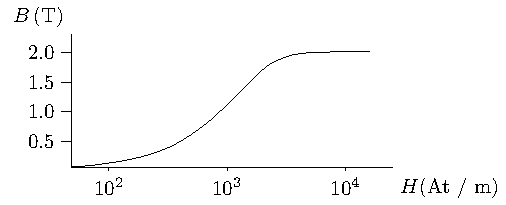
\includegraphics{figMagneticCircuitsM5curve}
\caption{$M5$ سٹیل کی $0.3048$ ملی میٹر موٹی پتری کا خط۔ میدانی شدت کا پیمانہ لاگ ہے۔}
\label{شکل_مقناطیسی_ادوار_ایم_پانچ_پتری_کا_خط}
\end{figure}

مختلف \عددیء{H} کے لئے  شکل \حوالہ{شکل_مقناطیسی_چال}-ب حاصل کر کے ایک ہی کاغذ پر کھینچنے کے بعد ان تمام کے  \عددیء{b} نقطے جوڑنے سے شکل \حوالہ{شکل_مقناطیسی_ادوار_ایم_پانچ_پتری_کا_خط} میں دکھایا \عددیء{B-H} خط حاصل ہوتا ہے۔ شکل \حوالہ{شکل_مقناطیسی_ادوار_ایم_پانچ_پتری_کا_خط} میں ٹرانسفارمروں میں استعمال ہونے والی  \عددیء{0.3048}  ملی میٹر موٹی \عددیء{M5} مرکز کی پتری کا \عددیء{B-H} خط دکھایا گیا ہے۔ اس خط میں موجود مواد جدول \حوالہ{جدول_مقناطیسی_ادوار_کثافت_بہاو_بالمقابل_شدت}  میں بھی دیا گیا ہے۔عموماً مقناطیسی مسائل حل کرتے ہوئے شکل \حوالہ{شکل_مقناطیسی_چال} کی جگہ شکل \حوالہ{شکل_مقناطیسی_ادوار_ایم_پانچ_پتری_کا_خط} کی طرح کا خط استعمال کیا جاتا ہے۔دھیان رہے کہ اس خط میں \عددیء{H}  کا پیمانہ \اصطلاح{لاگ}\حاشیہب{log} میں دکھایا گیا ہے۔

لوہا نما مقناطیسی اشیاء پر لاگو مقناطیسی شدت بڑھانے سے کثافتِ مقناطیسی بہاو بڑھنے کی شرح بتدریج کم ہوتی جاتی ہے حتیٰ کہ آخر کار یہ شرح خلاء کی شرح  \عددیء{\mu_0} رہ جاتی ہے یعنی
\begin{align}
\frac{\Delta B}{\Delta H}=\mu_0
\end{align}
اس اثر کو \اصطلاح{سیرابیت}\فرہنگ{سیرابیت}\حاشیہب{saturation}\فرہنگ{saturation} کہتے ہیں۔یہ شکل \حوالہ{شکل_مقناطیسی_ادوار_ایم_پانچ_پتری_کا_خط}  میں واضح ہے۔

شکل \حوالہ{شکل_مقناطیسی_چال} سے واضح ہے کہ \عددیء{H} کے کسی بھی قیمت پر \عددیء{B} کے  دو ممکنہ قیمتیں ہیں۔ اگر مقناطیسی بہاو بڑھ رہا ہو تو گراف میں نیچے سے اُوپر جانے والی لکیر اِس میں \عددیء{B} اور \عددیء{H} کے تعلق کو پیش کرتی ہے اور اگر مقناطیسی بہاو کم ہو رہا ہو تو اوپر سے نیچے آنے والی لکیر اِس تعلق کو پیش کرتی ہے۔  چونکہ \عددیء{\mu=B/H} ، لہٰذا \عددیء{B} کے  مقدار تبدیل ہونے سے \عددیء{\mu} بھی تبدیل ہوتی ہے۔ باوجود اِس کے ہم مقناطیسی دوروں میں یہ تصور کرتے ہیں کہ \عددیء{\mu} ایک مقررہ ہے۔ یہ تصور کر لینے سے عموماً جواب پر زیادہ اثر نہیں پڑتا۔
%
\ابتدا{مثال}
شکل \حوالہ{شکل_مقناطیسی_ادوار_ایم_پانچ_پتری_کا_خط}  یا اس کے مساوی جدول \حوالہ{جدول_مقناطیسی_ادوار_کثافت_بہاو_بالمقابل_شدت} میں دیئے گئے مواد کو استعمال کرتے ہوئے شکل \حوالہ{شکل_مقناطیسی__کثافت_مقناطیسی_بہاو_اور_شدت}  کی خلاء میں ایک ٹسلا اور دو ٹسلا کثافتِ  مقناطیسی بہاو حاصل کرنے کے لئے درکار برقی رو معلوم کریں۔اس شکل میں
\begin{align*}
b=\SI{5}{\centi\meter},w=\SI{4}{\centi\meter},l_a=\SI{3}{\milli\meter},l_c=\SI{30}{\centi\meter},N=1000
\end{align*}
ہیں۔مرکز اور خلاء کی رقبہ عمودی تراش برابر لیں۔

حل: ایک ٹسلا کے لئے۔

 جدول \حوالہ{جدول_مقناطیسی_ادوار_کثافت_بہاو_بالمقابل_شدت}  سے ہم دیکھتے ہیں کہ مرکز میں \عددیء{1} ٹسلا  حاصل کرنے کے لئے  مرکز کو \عددیء{11.22}  ایمپیئر-چکر فی \عددیء{H} میٹر  درکار ہے۔یوں \عددیء{30} سم لمبے مرکز کو \عددیء{0.3\times 11.22=3.366}  ایمپیئر چکر درکار ہیں۔

خلاء کو
\begin{align*}
H=\frac{B}{\mu_0}=\frac{1}{4\pi 10^{-7}}=\num{795671}
\end{align*}
ایمپیئر-چکر فی میٹر درکار ہیں۔لہٰذا \عددیء{ 3 } ملی میٹر لمبی خلاء کو \عددیء{0.003 \times 795671=2387} ایمپیئر چکر درکار ہیں۔یوں کُل ایمپیئر-چکر \عددیء{3.366+2387=2390.366} ہیں جن سے 
\begin{align*}
i=\frac{2390.366}{1000}=\SI{2.39}{\ampere}
\end{align*}	
حاصل ہوتی ہے۔

حل: دو ٹسلا کے لئے۔

جدول \حوالہ{جدول_مقناطیسی_ادوار_کثافت_بہاو_بالمقابل_شدت} سے ہم دیکھتے ہیں کہ مرکز میں \عددیء{2} ٹسلا  حاصل کرنے کے لئے  مرکز کو \عددیء{10000} ایمپیئر-چکر فی میٹر \عددیء{H} درکار ہے۔یوں \عددیء{30} سم لمبے مرکز کو \عددیء{0.3 \times 10000=3000} ایمپیئر چکر درکار ہیں۔خلاء کو
\begin{align*}
H=\frac{B}{\mu_0}=\frac{2}{4\pi 10^{-7}}=\num{1591342}
\end{align*}
ایمپیئر-چکر فی میٹر درکار ہیں۔لہٰذا \عددیء{3} ملی میٹر لمبی خلاء کو  \عددیء{0.003 \times 1591342=4774}  ایمپیئر چکر درکار ہیں۔یوں کُل ایمپیئر-چکر \عددیء{3000+4774=7774}	ہیں جن سے 
\begin{align*}
i=\frac{7774}{1000}=\SI{7.774}{\ampere}
\end{align*}
حاصل ہوتی ہے۔

اس مثال میں مقناطیسی سیرابیت کے اثرات واضح ہیں۔ 
\انتہا{مثال}
%
\begin{table}
\begin{tabular}{l l l l   l l l l   l l l l}
$H$&$B$&$H$&$B$&$H$&$B$&$H$&$B$&$H$&$B$&$H$&$B$\\
\hline\\
9000&1.998&1000&1.852&           200&1.720 &30&1.480               &9&0.700&  0&0.000    \\
10000&2.000&2000&1.900&         300&1.752 &40&1.540           &10&0.835&  2&0.040    \\
20000&2.020&3000&1.936&         400&1.780 &50&1.580          &11.22&1.000&  3&0.095    \\
30000&2.040& 4000&1.952&        500&1.800 &60&1.601         &12.59&1.100 &  4&0.160    \\
40000&2.048&5000&1.968&         600&1.810 &70&1.626          &14.96&1.200&   5&0.240    \\
50000&2.060&6000&1.975&         700&1.824 &80&1.640         &17.78&1.300&  6&0.330    \\
60000&2.070&7000&1.980&         800&1.835  &90&1.655         &20&1.340&  7&0.440    \\
 70000&2.080&8000&1.985&        900&1.846 &100&1.662          &23.77&1.400& 8&0.560    \\
\hline
\end{tabular}
\caption{مقناطیسی بہاو بالمقابل شدت}
\label{جدول_مقناطیسی_ادوار_کثافت_بہاو_بالمقابل_شدت}
\end{table}
%

\حصہ{ہیجان شدہ لچھا}
عموماً بدلتی رو بجلی میں برقی دباؤ اور مقناطیسی بہاو سائن نما ہوتے ہیں یعنی یہ وقت کے ساتھ \عددیء{\sin \omega t} یا \عددیء{\cos \omega t} کا تعلق رکھتے ہیں۔ اِس سبق میں ہم بدلتی رو سے لچھے کو ہیجان کرنا اور اس سے نمودار ہونے والے برقی توانائی  کے ضیاع  کا تذکرہ  کریں گے۔ ہم فرض کرتے ہیں کہ مرکز میں کثافتِ مقناطیسی بہاو 
\begin{align}
B=B_0 \sin \omega t
\end{align}
یوں مرکز میں بدلتا مقناطیسی بہاو \عددیء{\varphi}
\begin{align}
\varphi=A_c B=A_c B_0 \sin \omega t=\phi_0 \sin \omega t
\end{align}
ہے۔اس مساوات میں مقناطیسی بہاو کا حیطہ  \عددیء{\mp\phi_0} اور \عددیء{B} کا حیطہ \عددیء{\mp B_0} کے مابین تبدیل ہوتے ہیں۔\عددیء{A_c} مرکز کا رقبہ عمودی تراش ہے جو ہر جگہ یکساں ہے ۔\عددیء{\omega = 2 \pi f} ہے جہاں \عددیء{f} تعدد ہے۔

فیراڈے کے قانون یعنی مساوات \حوالہ{مساوات_مقناطیسی_دور_فیراڈے_قانون}  کے تحت اس مقناطیسی بہاو کی وجہ سے لچھے میں \عددیء{e(t)} برقی دباؤ  پیدا ہو گی۔
\begin{gather}
\begin{aligned}
e(t)&=\frac{\partial \lambda}{\partial t}\\
&=\omega N \phi_0 \cos \omega t \\
&=\omega N A_c B_0 \cos \omega t\\
&=E_0 \cos \omega t
\end{aligned}
\end{gather}
جس کا حیطہ
\begin{align}
E_0=\omega N \phi_0=2 \pi f N A_c B_0
\end{align}
ہے۔\عددیء{e(t)} کو \اصطلاح{امالی برقی دباؤ}\فرہنگ{امالی برقی دباؤ}\حاشیہب{induced voltage}\فرہنگ{induced voltage} کہتے ہیں۔ 

ہم بدلتی رو مقداروں کے مربع کی اوسط کے جزر  میں دلچسپی رکھتے ہیں۔یہی ان مقداروں کی \اصطلاح{موثر}\فرہنگ{موثر}\حاشیہب{root mean square, rms}\فرہنگ{rms} قیمت ہوتی ہے۔ جیسا صفحہ \حوالہصفحہ{مساوات_بنیادی_سائن_نما_کی_موثر_قیمت} پر مساوات \حوالہ{مساوات_بنیادی_سائن_نما_کی_موثر_قیمت}  میں دیکھا گیا ہے، ایک سائن نما  موج کی موثر قیمت اس کے حیطہ کے  \عددیء{1/\sqrt{2}} گنّا ہوتی ہے لہٰذا 
\begin{align}\label{مساوات_مقناطیسی_دور_پیدا_دباؤ_موثر_قیمت}
E_{rms}=\frac{E_0}{\sqrt{2}}=\frac{2 \pi f N A_c B_0}{\sqrt{2}}=4.44 f N A_c B_0
\end{align}
یہ مساوات بہت اہمیت رکھتی ہے اور ہم اس کو بار بار استعمال کریں گے۔بدلتی برقی دباؤ یا بدلتی برقی رو کی مقدار کی جب بھی ذکر ہو، یہ ان کی مربع کی اوسط کے جزر  یعنی اس کے موثر قیمت  کا ذکر ہوتا ہے۔پاکستان میں گھریلو برقی دباؤ \عددیء{220} وولٹ ہے۔اس کا مطلب ہے کہ اس برقی دباؤ کی موثر قیمت \عددیء{220} وولٹ ہے۔ چونکہ یہ سائن نما ہے لہٰذا اس کی چوٹی \عددی{\sqrt{2} \times 220=311} وولٹ ہے۔
%
\ابتدا{مثال}\شناخت{مثال_مقناطیسی_دور_محرک_برقی_رو_کا_گراف}
شکل \حوالہ{شکل_مقناطیسی__سادہ_مقناطیسی_دور_بغیر_درز} میں \عددیء{27} چکر ہیں۔ مرکز کی لمبائی \عددیء{30 } سم جبکہ اس کا رقبہ عمودی تراش \عددیء{229.253} مربع سم ہے۔لچھے  میں گھریلو \عددیء{220} وولٹ موثر برقی دباؤ سے ہیجان  پیدا کیا جاتا ہے۔جدول \حوالہ{جدول_مقناطیسی_ادوار_کثافت_بہاو_بالمقابل_شدت} کی مدد سے مختلف برقی دباؤ پر محرک برقی رو معلوم کریں اور اس کا خط کھینچیں۔

حل:
	گھریلو برقی دباؤ \عددیء{50} ہرٹز کی سائن نما موج ہوتی ہے یعنی
\begin{align}
v=\sqrt{2} \times 220 \cos (2 \pi  50 t)
\end{align}
مساوات \حوالہ{مساوات_مقناطیسی_دور_پیدا_دباؤ_موثر_قیمت}  کی مدد سے ہم کثافتِ مقناطیسی بہاو کی چوٹی حاصل کرتے ہیں
\begin{align}
B_0=\frac{220}{4.44 \times 50 \times 27 \times 0.0229253}=\SI{1.601}{\tesla}
\end{align}
لہٰذا مرکز میں کثافتِ مقناطیسی بہاو صفر سے \عددیء{\mp1.601}  ٹسلا کے درمیان تبدیل ہوتی رہتی ہے۔یوں مرکز میں کثافتِ مقناطیسی بہاو کی مساوات یہ ہو گی
\begin{align}\label{مساوات_مقناطیسی_دور_سائن_نما_کثافت_بہاو}
B=1.601 \sin \omega t
\end{align}
ہم فہرست کی مدد سے کثافتِ مقناطیسی بہاو کے  \عددی{0} سے \عددیء{1.601} ٹسلا کے درمیان مختلف قیمتوں پر درکار محرک برقی رو \عددیء{i_{\phi}} معلوم کرنا چاہتے ہیں۔ہم مختلف \عددیء{B} پر جدول \حوالہ{جدول_مقناطیسی_ادوار_کثافت_بہاو_بالمقابل_شدت} سے مرکز کی \عددیء{H} حاصل کریں گے جو کہ ایک میٹر لمبی مرکز کے لئے درکار ایمپیئر-چکر دیتی ہے۔اس سے \عددیء{30} سم لمبی مرکز کے لئے درکار ایمپیئر-چکر  حل کر کے برقی رو حاصل کریں گے۔

%
\begin{table}
\begin{tabular}{l l l l l | l l l l l}
$i_{\varphi}=\frac{0.3 H}{27}$&$0.3H$&$H$&$B$&$\omega t$&$i_{\varphi}=\frac{0.3 H}{27}$&$0.3H$&$H$&$B$&$\omega t$\\
\hline\\
0.000&0.000&0&0.000&0.000&0.125&3.366&11.22&1.000&0.675\\
0.022&0.600&2&0.040&0.025&0.140&3.777&12.59&1.100&0.757\\
0.033&0.900&3&0.095&0.059&0.166&4.488&14.96&1.200&0.847\\
0.044&1.200&4&0.160&0.100&0.198&5.334&17.78&1.300&0.948\\
0.056&1.500&5&0.240&0.150&0.222&6.000&20&1.340&0.992\\
0.067&1.800&6&0.330&0.208&0.264&7.131&23.77&1.400&1.064\\
0.078&2.100&7&0.440&0.278&0.333&9.000&30&1.480&1.180\\
0.089&2.400&8&0.560&0.357&0.444&12.000&40&1.540&1.294\\
0.100&2.700&9&0.700&0.453&0.556&15.000&50&1.580&1.409\\
0.111&3.000&10&0.835&0.549&0.667&18.000&60&1.601&1.571\\
\hline
\end{tabular}
\caption{محرک برقی رو}
\label{جدول_مقناطیسی_ادوار_محرک_برقی_رو_بالمقابل_کثافت_بہاو}
\end{table}

جدول \حوالہ{جدول_مقناطیسی_ادوار_محرک_برقی_رو_بالمقابل_کثافت_بہاو}  مختلف کثافتِ مقناطیسی بہاو کے لئے درکار محرک برقی رو دیتی ہے۔جدول میں  ہر \عددیء{B} کی قیمت پر  \عددیء{\omega t} مساوات \حوالہ{مساوات_مقناطیسی_دور_سائن_نما_کثافت_بہاو}  کی مدد سے حاصل کی گئی ہے۔\عددیء{\omega t} بالمقابل محرک برقی رو کا خط شکل \حوالہ{شکل_مقناطیسی_ادوار_ہیجان_رو_چال_نظرانداز} میں دیا گیا ہے۔
\انتہا{مثال}
%
\begin{figure}
\centering
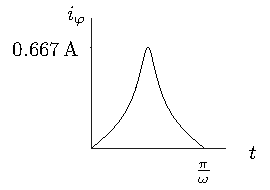
\includegraphics{figExcitationCurrentFromBHbrillouinCurveNeglectingHysterisisA}
\caption{$M5$ پتری کے مرکز میں $1.6$ ٹسلا تک ہیجان پیدا کرنے کے لئے درکار ہیجان انگیز برقی رو۔}
\label{شکل_مقناطیسی_ادوار_ہیجان_رو_چال_نظرانداز}
\end{figure}
برقی لچھے میں برقی دباؤ سے ہیجان پیدا کیا جاتا ہے۔ہیجان شدہ لچھے میں برقی رو کی وجہ سے  مرکز میں مقناطیسی بہاو پیدا ہوتا ہے۔ اس برقی رو \عددیء{i_{\varphi}} کو \اصطلاح{ہیجان انگیز برقی رو}\فرہنگ{برقی رو!ہیجان انگیز}\حاشیہب{excitation current}\فرہنگ{excitation current}  کہتے ہیں۔

مثال \حوالہ{مثال_مقناطیسی_دور_محرک_برقی_رو_کا_گراف} میں ہیجان انگیز برقی رو معلوم کی گئی جسے شکل \حوالہ{شکل_مقناطیسی_ادوار_ہیجان_رو_چال_نظرانداز} میں دکھایا گیا۔اسے حاصل کرتے وقت \اصطلاح{مقناطیسی چال}\فرہنگ{مقناطیسی چال}\حاشیہب{hysteresis} کو نظر انداز کیا گیا۔شکل \حوالہ{شکل_مقناطیسی_ادوار_ہیجان_رو_بشمول_اثر_چال} میں ہیجان انگیز برقی رو \عددیء{i_\varphi} دکھائی گئی ہے جو مقناطیسی چال کو مدِ نظر رکھ کر حاصل کی گئی ہے۔ اس کو سمجھنا نہایت ضروری ہے۔
\begin{figure}
\centering
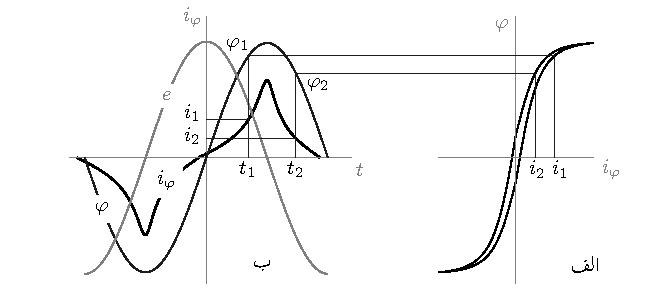
\includegraphics{figExcitationCurrentFromBHbrillouinCurveA}
\caption{ہیجان انگیز برقی رو۔}
\label{شکل_مقناطیسی_ادوار_ہیجان_رو_بشمول_اثر_چال}
\end{figure}
%
\begin{figure}
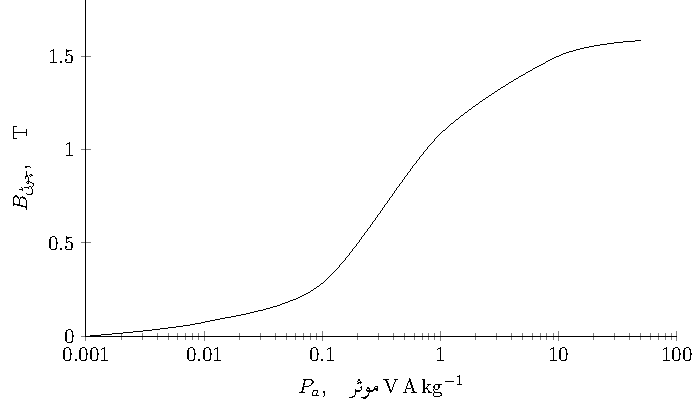
\includegraphics{figMagneticCircuitsVoltAmperePerKgVersusFluxDensity}
\caption{پچاس ہرٹز پر \عددیء{0.3} ملی میٹر موٹی پتری کے لئے درکار موثر وولٹ-امپیئر فی کلوگرام مرکز}
\label{شکل_مقناطیسی_دور_درکار_ہیجان_وولٹ_ایمپیئر}
\end{figure}
شکل \حوالہ{شکل_مقناطیسی_ادوار_ہیجان_رو_بشمول_اثر_چال}-الف میں  مقناطیسی چال کا خط ہے۔چونکہ
\begin{gather}
\begin{aligned}
H l& =N i\\
\varphi&=B A_c
\end{aligned}
\end{gather}
ہیں لہٰذا مقناطیسی چال کے  خط کو \عددیء{\varphi-i_{\varphi}} کا خط لکھا جا سکتا ہے۔شکل \حوالہ{شکل_مقناطیسی_ادوار_ہیجان_رو_بشمول_اثر_چال}-ب مرکز میں سائن نما مقناطیسی بہاو \عددیء{\varphi} دکھا رہا ہے۔سائن نما مقناطیسی بہاو کی موج وقت کے ساتھ تبدیل ہوتی ہے۔لمحہ \عددیء{t_1} پر اس موج کی مقدار  \عددیء{\varphi_1} ہے۔مقناطیسی بہاو \عددیء{\varphi_1} حاصل کرنے کے لئے درکار ہیجان انگیز برقی رو \عددیء{i_1} شکل-الف سے حاصل کی جا سکتی ہے۔اسی  ہیجان انگیز برقی رو کو شکل-ب میں  لمحہ \عددیء{t_1} پر دکھایا گیا ہے۔ 

دھیان رہے کہ لمحہ \عددیء{t_1} پر مقناطیسی بہاو بڑھ رہی ہے لہٰذا مقناطیسی چال کے خط کا صحیح حصہ استعمال کرنا ضروری ہے۔شکل \حوالہ{شکل_مقناطیسی_ادوار_ہیجان_رو_بشمول_اثر_چال}-الف میں  \عددیء{\varphi-i_{\varphi}}  کے خط میں گھڑی کے الٹی جانب گھومتے ہوئے یوں نیچے سے اوپر جاتا ہوا حصہ استعمال کیا گیا ہے۔مقناطیسی بہاو بڑھنے کی صورت میں شکل \حوالہ{شکل_مقناطیسی_چال}-ب میں نیچے سے اوپر جاتے  ہوئے حصے پر تیر کا نشان صحیح سمت دکھلاتا ہے۔اسی طرح مقناطیسی بہاو گھٹنے کی صورت میں اوپر سے نیچے جاتے حصے پر تیر کا نشان صحیح حصہ دکھلاتا ہے۔

 لمحہ \عددیء{t_2} پر مقناطیسی بہاو گھٹ رہی ہے۔اس لمحہ پر مقناطیسی بہاو \عددیء{\varphi_2} ہے اور اسے حاصل کرنے کے لئے درکار ہیجان انگیز برقی رو \عددیء{i_2} ہے۔

اگر اسی طرح مختلف لمحات پر درکار ہیجان انگیز برقی رو حاصل کی جائے تو ہمیں شکل \حوالہ{شکل_مقناطیسی_ادوار_ہیجان_رو_بشمول_اثر_چال}-ب میں دکھائی گئی  \عددیء{i_{\varphi}} کا خط ملے گی۔یہ ایک غیر سائن نما خط ہے۔

آپ جانتے ہیں کہ اگر \عددیء{\varphi=\phi_0 \sin \omega t} ہو تب برقی دباؤ \عددیء{e=N \tfrac{\dif \varphi}{\dif t}=N \phi_0 \omega \cos \omega t} ہو گا۔شکل \حوالہ{شکل_مقناطیسی_ادوار_ہیجان_رو_بشمول_اثر_چال}-ب میں اس برقی دباؤ کو بھی دکھایا گیا ہے۔آپ دیکھ سکتے ہیں کہ مقناطیسی بہاو برقی دباؤ سے \عددیء{90 \degree} پیچھے ہے۔

 اگر مرکز میں  \عددیء{B=B_0 \sin \omega t} ہو  تو اِس میں \عددیء{H} اور \عددیء{i_{\varphi}} ایک غیر سائن نما شکل اختیار کر لیتے ہیں۔ اس صورت میں  اِن کے موثر قیمتوں \عددیء{H_{c,rms}} اور  \عددیء{i_{\varphi,rms}} کا تعلق یہ ہے
\begin{align}\label{مساوات_مقناطیسی_دور_دباؤ_برابر_شدت_ضرب_لمبائی}
N i_{\varphi,rms}=l_c H_{c,rms}
\end{align}
مساوات \حوالہ{مساوات_مقناطیسی_دور_پیدا_دباؤ_موثر_قیمت}   اور مساوات \حوالہ{مساوات_مقناطیسی_دور_دباؤ_برابر_شدت_ضرب_لمبائی}  سے ملتا ہے
\begin{align}\label{مساوات_مقناطیسی_دور_درکار_دباؤ_ضرب_رو}
E_{rms} i_{\varphi,rms}=\sqrt{2} \pi f B_0 H_{c,rms} A_c l_c
\end{align}
یہاں \عددیء{A_c l_c} مرکز کا حجم ہے۔ لہٰذا یہ مساوات ہمیں \عددیء{A_c l_c} حجم کی مرکز  کو \عددیء{B_0} کثافتِ مقناطیسی بہاو تک ہیجان کرنے کے لئے درکار \عددیء{E_{rms} i_{\varphi,rms}} بتلاتا ہے۔ ایک مقناطیسی مرکز جس کا حجم  \عددیء{A_c l_c} اور  میکانی کثافت  \عددیء{\rho_c} ہو، اس کی کمیت \عددیء{m_c=\rho_c A_c l_c} ہو گی۔ یوں ہم، ایک کلوگرام  مرکز، کے لئے مساوات \حوالہ{مساوات_مقناطیسی_دور_درکار_دباؤ_ضرب_رو}   کو یوں لکھ سکتے ہیں
\begin{align}
P_a=\frac{E_{rms} i_{\varphi,rms}}{m_c}=\frac{\sqrt{2} \pi f}{\rho_c} B_0 H_{c,rms}
\end{align}
دیکھا جائے تو کسی ایک تعدد  \عددیء{f} پہ \عددیء{P_a} کی قیمت صرف مرکز اور اس میں \عددیء{B_0} یعنی \عددیء{B_{\textup{چوٹی}}} پر منحصر ہے، چونکہ \عددیء{H_{c,rms}} خود \عددیء{B_0} پر منحصر ہے۔ اِسی وجہ سے مرکز بنانے والے، اکائی کمیت کے مرکز میں مختلف \عددیء{B_{\textup{چوٹی}}} پیدا کرنے کیلئے درکار \عددیء{E_{rms} i_{\varphi,rms}}، کو \عددیء{B_0} اور \عددیء{P_a} کے مابین گراف کی شکل میں دیتے ہیں۔مرکز کی \عددیء{0.3} ملی میٹر موٹی پتری کے لئے ایسا گراف  شکل \حوالہ{شکل_مقناطیسی_دور_درکار_ہیجان_وولٹ_ایمپیئر} میں دکھایا گیا ہے۔
